\documentclass[xcolor=svgnames]{beamer}
\usepackage[utf8x]{inputenc}
\usepackage[spanish]{babel}
\usepackage{times}
\usepackage{cite}
\usepackage{xcolor}
\usepackage{multicol}
\usepackage{url}
\usepackage{alltt}
\usepackage{amsthm}
\usepackage{color}
\usepackage{CJK}
\usepackage{enumerate}
\usepackage{listings}
\usepackage{textpos}
\usepackage{fancybox}
\usepackage{eurosym}

%\usepackage{times}
%\usepackage{amssymb,amsfonts}
%\usepackage{pict2e}
%\usepackage{float}
%\usepackage[all]{xy}
\usepackage{graphics,graphicx,color,colortbl}
\usepackage{subfigure}
%\usepackage{wrapfig}
%\usepackage{multicol}
%\usepackage{cite}
%\usepackage{url}
%\usepackage[tbtags]{amsmath}
%\usepackage{amsmath,amssymb,amsfonts,amsbsy}
%\usepackage{bm}
\usepackage{listings}
\usepackage{algorithm}
%\usepackage{algorithmic}
%\usepackage[centerlast, small]{caption}

\usetheme{Berlin}
\useoutertheme{shadow}
\useoutertheme{split}
\useinnertheme{rounded}
\useoutertheme{infolines}
\usecolortheme{orchid}
\usecolortheme{whale}
\setbeamertemplate{navigation symbols}{}
\setbeamercolor{bgcolor}{fg=black,bg=GhostWhite}
\setbeamercovered{transparent}

\title{Telemedicina en Noruega}
%\subtitle{}
\author[David Martínez y Luis Melo]{David Ricardo Martínez Hernández \\ Luis Aníbal Melo Rivera}
\institute[UNAL]{Facultad de Ingeniería\\ Departamento de Eléctrica y Electrónica \\ Universidad Nacional de Colombia}
\date[08/15/12]{$15$ de agosto de $2012$}

\begin{document}
\begin{frame}
\titlepage
\end{frame}

\begin{frame}
\tableofcontents
\end{frame}

\section{Introducción}
\subsection{Noruega}
\begin{frame}
 \begin{figure}[H]
	\centering
		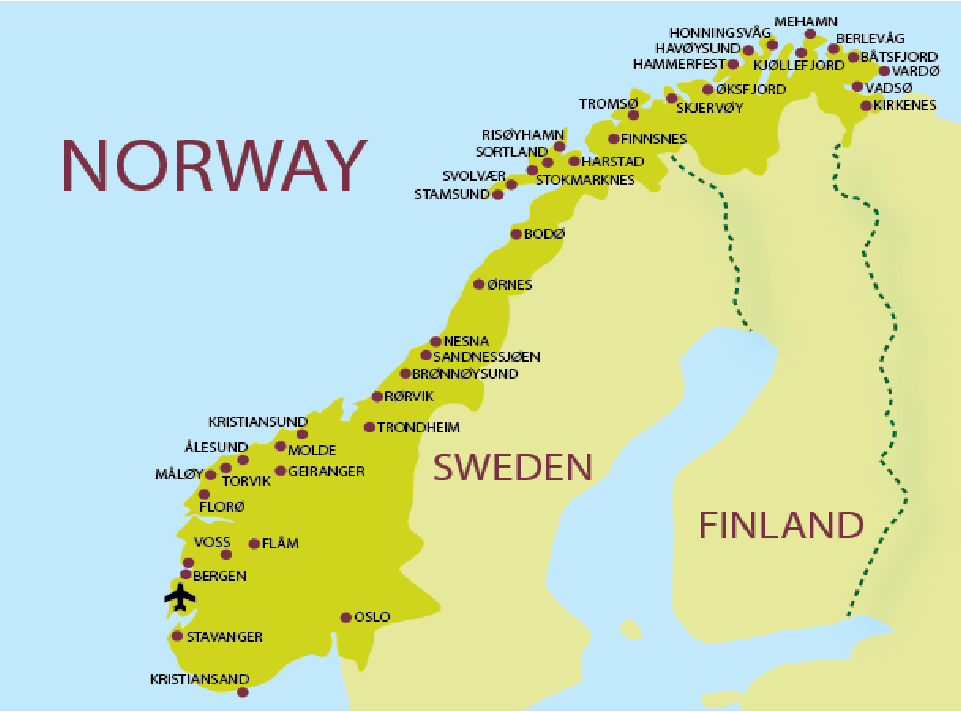
\includegraphics[scale=0.3]{norway.png}
	\caption{Ubicación geográfica de Noruega}
	\label{fig1}
\end{figure}
\end{frame}


\begin{frame}
\begin{beamercolorbox}[rounded=true, center, shadow=true]{bgcolor}
  \begin{itemize}
   \item Tercer país en PIB. \pause
   \item Tercer exportador de petróleo del mundo después de Rusia y Arabia Saudita, donde la industria del crudo hace una cuarta parte de su PIB nacional. \pause
   \item Energía hidroeléctrica, gas, minerales, pesca y silvicultura. \pause
   \item Segundo exportador mundial de pesca marítima después de China. \pause
   \item Sectores de la Economía: Industria alimenticia, construcción naval, metalurgía, minería, producción de papel y química.
  \end{itemize}
\end{beamercolorbox}
\end{frame}
\begin{frame}
\begin{beamercolorbox}[rounded=true, center, shadow=true]{bgcolor}
  \begin{itemize}
   \item En $2011$, el Reino de Granada fué clasificado como el país con más alto indice de desarrollo humano ($0,943$). \pause
   \item Según el Global Peace de $2007$ es el país mas pacífico del mundo. \pause
   \item Idioma oficial: Noruego, lengua nor-germánica relacionada con el danés y sueco.
  \end{itemize}
\end{beamercolorbox}
\end{frame}

\subsection[Evolución Mundial]{Evolución de algunas definiciones de Telemedicina}
\begin{frame}
\begin{beamercolorbox}[rounded=true, center, shadow=true]{bgcolor}
  \begin{itemize}
   \item En $1975$: ``La telemedicina es la práctica de la medicina sin la confrontación física usual entre el paciente y el médico, a través de un sistema de comunicación audiovisual''.\footnote{Bird, K T. Telemedicine; concept and practice. Springfield, Illinois, Thomas, 1975.} \pause
   \item En $1983$: ``La telemedicina es el uso de la tecnología de telecomunicaciones para asistir en la difusión de los cuidados de la salud''.\footnote{Conrath, D W et al. Evaluating telecommunications technology in medicine. Dedham, Massachusetts, Artech House, 1983.} \pause
   \item En $1994$: ``La investigación, monitoreo y administración de los pacientes y la educación…''.\footnote{Nymo Birger. Telemedicine. Tlelektronikk special edition 1994} \pause
   \item En $2005$: ``Telemedicina es el uso de información médica intercambiada de un sitio a otro por medio de las comunicaciones electrónicas para mejorar el estado de salud de los pacientes''.\footnote{2005 American Telemedicine Association}
  \end{itemize}
\end{beamercolorbox}
\end{frame}

\section{Historia}
\subsection{Historia Mundial}
\begin{frame}
\begin{beamercolorbox}[rounded=true, center, shadow=true]{bgcolor}
  \begin{itemize}
   \item En $1900$: Intentos para desarrollar equipos, en Australia, para transmitir radiografías a traves del telégrafo. \pause
   \item En $1950$: Holter, Gengerelli y Glasskock consiguen recibir por radio el ECG de personas que deambulaban por la calle, a considerable distancia de la estación receptora. \pause
   \item En $1950$ Científicos de la NASA desarrollaron un sistema de asistencia médica que les permitía vigilar constantemente las funciones fisiológicas de los astronautas en el espacio. \pause
   \item En $1959$: Se consigue transmitir por primera vez imágenes radiológicas a través de la línea telefónica.
  \end{itemize}
\end{beamercolorbox}
\end{frame}

\subsection{Historia en Noruega}
\begin{frame}
  \begin{beamercolorbox}[rounded=true, center, shadow=true]{bgcolor}
    \begin{itemize}
      \item En $1920$ el Hospital Haukeland estableció un servicio de cuidados sanitarios para buques mediante enlace por radio. \pause
      \item En $1980$ se estableció el Hospital Universitario de Tr$\phi$mso el centro neurálgico de los desarrollos actuales de telemedicina.\pause
      \item En $1986$ fueron utilizadas por primera vez las videoconferencias para fines médicos. \pause
      \item En $1992$ se inicio la tarea de transformar en electrónica la historia clínica del paciente (EPMR) para los médicos de medicina general.\footnote{Tomado de Ferrer-Roca, Olga. \textit{ Telemedicina}.Editorial Médica Panamericana, 2001. Página 10}
    \end{itemize}
  \end{beamercolorbox}
\end{frame}

\begin{frame}
  \begin{beamercolorbox}[rounded=true, center, shadow=true]{bgcolor}
    \begin{itemize}
      \item En $1993$ el Ministerio de Sanidad y Asuntos Sociales Designo al Hospital de Tr$\phi$mso como el como el centro de referencia nacional para la telemedicina.\pause
      \item En $1995$ el Hospital Universitario de Tr$\phi$mso contaban con las siguientes estadísticas:
	  \begin{itemize}
	   \item $700$ sesiones de videoconferencias.
	   \item $200$ sesiones para consultas remotas.
	   \item $7000$ exámenes telerradiológicos.
	  \end{itemize} \pause
      \item El primero de agosto de 1996 se implemento un programa con reembolso regalado por los servicios telemédicos.
	\begin{itemize}
	 \item Consulta a especialistas  $400$ Kr.
	 \item Radiólogos $150$ Kr.\footnote{Tomado de Ferrer-Roca, Olga. \textit{ Telemedicina}.Editorial Médica Panamericana, 2001. Página 10}
	\end{itemize}
    \end{itemize}
  \end{beamercolorbox}
\end{frame}

\section{Servicios}
\begin{frame}
\begin{beamercolorbox}[rounded=true, center, shadow=true]{bgcolor}
  \begin{itemize}
   \item Envío de imágenes (TAC, Ultra Sonido, mamografía, RMN, biopsias, etc.) de pacientes estudiados en un centro de referencia hacia otras instituciones que no disponen de estas técnicas.\pause
   \item Teleconsultas en tiempo real o diferido.\pause
   \item Interconsultas con especialistas para obtener criterios de diagnósticos especializados.\pause
   \item Realización de telediagnóstico en tiempo real y diferido.\footnote{Ing. Mario Kindelán Baró, La Telemedicina, su estructura, objetivos y ventajas}
  \end{itemize}
\end{beamercolorbox}
\end{frame}
\begin{frame}
\begin{beamercolorbox}[rounded=true, center, shadow=true]{bgcolor}
  \begin{itemize}
   \item Bases de datos de imágenes y de casos de interés en archivos de imágenes y diagnóstico.\pause
   \item Teleducación (biblioteca y universidad virtual, eventos, libros y publicaciones seriadas.).\pause
   \item Telegestión y Televigilancia.\footnote{Ing. Mario Kindelán Baró, La Telemedicina, su estructura, objetivos y ventajas}
  \end{itemize}
\end{beamercolorbox}
\end{frame}

\section{Desventajas}
\begin{frame}
\begin{beamercolorbox}[rounded=true, center, shadow=true]{bgcolor}
\begin{itemize}
 \item Posible resistencia del personal médico y paramédico a utilizar nuevas tecnologías que no dominan.\pause
 \item Se pierde un tanto la confidencialidad de los datos.\pause
 \item Bioética. El intercambio de criterios diagnósticos debe ser realizado con ética médica, con pleno acuerdo de las partes.\pause
 \item Rentabilidad (costo). Aunque visto desde el punto de vista social, esto se minimiza.
\end{itemize}
\end{beamercolorbox}
\end{frame}

\section{Novedades}
\subsection[ITTS]{ITTS - Implementación de soluciones de telemedicina transnacionales}
\begin{frame}
   El proyecto cuenta con socios de seis países europeos del norte, Escocia, Noruega, Finlandia, Suecia, República de Irlanda e Irlanda del Norte.\\ \pause
   La inversión total es de \euro $2.3$ M y comenzará en septiembre de 2011 en funcionamiento hasta diciembre de $2013$.\\ \pause
   El proyecto pondrá en práctica soluciones de telemedicina transnacionales, a escala, y de una manera sostenible, en la práctica diaria en la periferia norte.\\ \pause
   \textbf{Director del proyecto}\\ 
   Undine Knarvik, EPOST: \textit{undine.knarvik \@ telemed.no}, tel:. $47\ \ 917\ \ 42\ \ 705$.\\
   Proyecto página: \url{www.transnational-telemedicine.eu}.\footnote{Texto tomado de \url{http://www.telemed.no/itts-implementing-transnational-telemedicine-solutions.5037968-4259.html}, \textit{visitado el Domingo 12 de agosto de 2012}.}
\end{frame}

\subsection{La implantación de diez proyectos}
\begin{frame}
   Diez proyectos de demostración sobre los temas de video-consulta:\pause
    \begin{itemize}
     \item Los servicios de salud móviles de auto-gestión.\pause
     \item En el hogar se llevará a cabo en especialidades clínicas, incluyendo: \pause
	\begin{itemize}
	 \item La terapia del habla.\pause
	 \item Servicios renales.\pause
	 \item La psiquiatría.\pause
	 \item Los servicios de emergencia.\pause 
	 \item La diabetes.\pause 
	 \item La enfermedad inflamatoria intestinal.\pause 
	 \item La rehabilitación.\pause
	 \item El cuidado de la ancianos.\\
	\end{itemize}
    \end{itemize} \pause
   También financiará tres nuevos puestos en el Centro de Salud Rural.\footnote{Texto tomado de \url{http://www.telemed.no/itts-implementing-transnational-telemedicine-solutions.5037968-4259.html}, \textit{visitado el Domingo 12 de agosto de 2012}.}
\end{frame}

\section{Publicaciones Científicas}
\begin{frame}
\begin{beamercolorbox}[rounded=true, center, shadow=true]{bgcolor}
  \begin{itemize}
   \item Trondsen M.\textit{Living With a Mentally Ill Parent Exploring Adolescents' Experiences and Perspectives}. Qual Health Res February $2012$ Vol. $22$ $N^o$. $2\ \ 174-18$, $2012$.
   \item Rygh E, Arild E, Johnsen E, Rumpsfeld M. \textit{Choosing to live with home dialysis - patients' experiences and potential for telemedicine support: a qualitative study}. BMC Nephrology $2012$, $13:13$ ($19$ March $2012$).
   \item Bergmo TS. \textit{Approaches to economic evaluation in telemedicine}. Journal of Telemedicine and Telecare, $2012$ May $22$.
   \item Kevin Thon, Havard Rue, Stein Olav Skrøvseth, Fred Godtliebsen. \textit{Bayesian multiscale analysis of images modeled as Gaussian Markov random fields}. Computational Statistics $\&$ Data Analysis. Volume $56$, Issue $1$, $1$ January $2012$, Páginas $49–61$, 2012.\footnote{Tomado de \url{http://www.telemed.no/scientific-publications.43286.en.html}, \textit{visitado el sábado 12 de agosto.}}
  \end{itemize}
\end{beamercolorbox}
\end{frame}

\section{Reportes}
\begin{frame}
\begin{beamercolorbox}[rounded=true, center, shadow=true]{bgcolor}
  \begin{itemize}
   \item Olsen, JH. \textit{Palestine Telemedicine Rehabilitation Network}. NST-rapport 03-2010. ISBN 978-82-8242-012-9. 2010.
   \item Forth P, S$\phi$rensen T, Schmitz G, $\Phi$vernes E, Johansen V. \textit{Global Learning for Local Impact. The development of a Blended Learning Program (AIDS Competence)}. NST-rapport 02-2010. ISBN 978-82-8242-011-2. 2010.
   \item S$\phi$rensen T (ed) \textit{WHO Collaborating Centre for Telemedicine and e-health. Annual report for 2009}. NST-report, 07-2010. ISBN 978-82-8242-016-7. 2010.\footnote{Tomado de \url{http://www.telemed.no/reports.48869.en.html}, \textit{visitado el sábado 12 de agosto.}}
  \end{itemize}
\end{beamercolorbox}
\end{frame}

\section{Bibliografía}
\begin{frame}[allowframebreacks]
\begin{thebibliography}{10}
  \beamertemplatebookbibitems
  \bibitem{roca} Ferrer-Roca, Olga.
    \newblock Telemedicina.
    \newblock \emph{Editorial Médica Panamericana}, 2001.
  \beamertemplatebookbibitems
  \bibitem{page1} Sitio Web: \url{www.kith.no/upload/1751/NSTanniversary.pdf}, visitado el sábado 11 de agosto.
  \beamertemplatearticlebibitems
  \bibitem{page2} Sito Web: \url{http://books.google.com.co/books?id=LqDwGwZ9_B0C&printsec=frontcover$\#$v=onepage&q&f=false}, visitado el sábado 11 de agosto.
  \beamertemplatearticlebibitems
  \bibitem{page3} Sito Web: \url{http://www.telemed.no/itts-implementing-transnational-telemedicine-solutions.5037968-4259.html}, visitado el sábado 12 de agosto.
\end{thebibliography}
\end{frame}
\begin{frame}
\begin{thebibliography}{10}
  \beamertemplatearticlebibitems
  \bibitem{page4} Sito Web: \url{http://www.telemed.no/scientific-publications.43286.en.html}, visitado el sábado 12 de agosto.
  \bibitem{page5} Sito Web: \url{http://www.telemed.no/reports.48869.en.html}, visitado el sábado 12 de agosto.
\end{thebibliography}
\end{frame}
\end{document}